\section{Testbed, runtimes, and controllers}
\label{sec:testbed}

\subsection{Process-per-vertex architecture}

Each vertex of a call graph runs as its own operating-system process with a gRPC server. The root vertex receives requests from an open-loop load generator running in a separate process. Edges are gRPC calls that carry the request payload and an absolute deadline in metadata. A run therefore involves one generator process, one process per vertex, and, in the sidecar phase, one proxy process per edge. Figure~\ref{fig:arch_dacshed} shows the harness and the admission gate that DAC-Shed installs in front of each vertex's worker pool. Every process is pinned to the same eight-core host, so the generator, the vertices, and the proxies compete for the same processors. That shared host is the reason for the quiet-host protocol in Section~\ref{sec:protocol}.

\begin{figure}[!t]
\centering
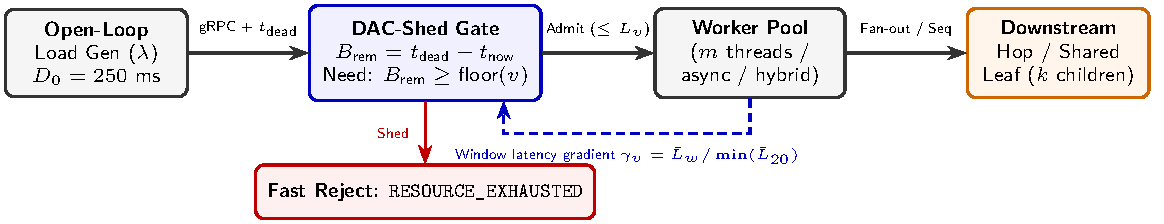
\includegraphics[width=\columnwidth]{arch_dacshed.pdf}
\caption{Single-host gRPC microservice harness and DAC-Shed admission gate. Each RPC carries its absolute deadline $t_{\text{dead}}$ in gRPC metadata. A vertex sheds a request before thread-pool queueing when the remaining budget is smaller than its critical-path floor, $B_{\text{rem}} < \text{floor}(v)$, or when in-flight work reaches the concurrency limit $L_v$. The latency gradient is computed over 50\,ms windows and updates $L_v$.}
\label{fig:arch_dacshed}
\end{figure}

\subsection{Concurrency runtimes}

Three runtimes are implemented, and they differ in where a thread is held. In the synchronous runtime, each vertex runs a bounded handler pool of eight worker threads. An in-flight request holds its handler thread across every downstream call, which is the situation the model describes. The asynchronous runtime uses \texttt{grpc.aio} with \texttt{uvloop}. A request never holds a thread across a downstream call, but its local work runs on the event loop, so the loop thread carries that work as well as protocol processing. The hybrid runtime keeps the asynchronous server and runs local work in a \texttt{ThreadPoolExecutor} with eight workers, so only the local processing time occupies the bounded pool. The downstream wait is performed on the loop and holds no thread.

The three runtimes therefore hold threads differently, and a fair comparison has to hold the offered load and the pool size fixed. The campaign does both. Phase~2 uses the same five offered loads for all three runtimes of each shape, so the curves can be compared point by point, and every runtime uses a pool of eight. The mechanism behind the differences is examined in Section~\ref{sec:runtimes}.

\subsection{Local work and service-time model}

Local work is modeled as an I/O-bound operation. Each vertex draws a lognormal service time with a mean of $10\,\mathrm{ms}$ and a log-standard deviation of $\sigma=0.5$, and $10\%$ of the drawn time is spent in a busy loop, so the model contributes CPU as well as waiting. The model has no database or disk component. Sleeps overshoot on the test machine by about $0.3\,\mathrm{ms}+0.44\,t$ for a requested sleep $t$, and the implementation shortens each sleep by that fitted amount. The fit is the calibration step that keeps the realized service time close to the drawn one. Request payloads are 64 bytes in every phase except Phase~3, which sweeps payloads from 64 bytes to 64\,KB.

The analytical model uses the same parameters. The pool size is $m_v=8$, the per-hop network cost is $\delta=0.5\,\mathrm{ms}$, and the CPU cost per visit used for the CPU capacity bound is $1.5\,\mathrm{ms}$.

\subsection{Open-loop load generation and latency measurement}

The load generator draws Poisson arrival offsets before each run starts. Each request has an intended send time, and its latency is measured from that intended time, not from the moment the request is actually sent. This is the coordinated-omission correction that open-loop measurement requires~\cite{schroeder2006open}. Generator lag, the difference between the intended and actual send times, is therefore added to the recorded latency, and it does not reduce the offered load.

Figure~\ref{fig:lag} shows the lag for all 180 Phase~1 runs. The median lag falls from about 1.8\,ms at 19\,req/s to 0.3\,ms at 312\,req/s, and the median per-run P99 lag stays between 1.6 and 3.8\,ms across load levels. Lag therefore falls as load rises, which does not look like generator saturation. We attribute the residual lag to timer and scheduler jitter, which we did not measure separately. Each run lasts 90\,s, and the first 10\,s are excluded from the statistics. Each request is recorded with its outcome (success, error, or timeout), its latency, and its generator lag. Per-vertex hop records are kept for one request in ten. Every run also records process CPU counters and host CPU counters at a sampling interval of $0.5\,\mathrm{s}$, together with a host-noise probe taken before the run.

\begin{figure}[t]
  \centering
  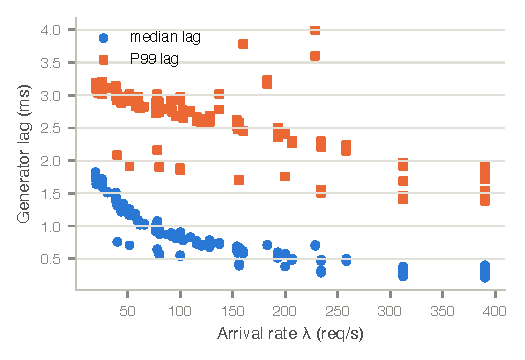
\includegraphics[width=\columnwidth]{fig06.pdf}
  \caption{Generator lag against offered rate, one point per run for all 180 Phase~1 runs. Circles show the median lag of a run and squares its P99 lag.}
  \label{fig:lag}
\end{figure}

\subsection{Sidecar emulation and tracing}
\label{sec:sidecar}

The sidecar in Phase~3 is a bytes-level pass-through process inserted in front of one vertex on each edge. It forwards the raw request and response unchanged, so it adds one hop and one byte copy, but it does not parse the protocol buffer. Its cost is measured from the caller's side, as the difference between the caller's wall time and the callee's own hop time, and from the proxy's own process CPU. The emulation is in-process and is not Envoy. The name ``sidecar'' refers to the cost structure of a proxy on the request path, not to a deployed mesh.

Tracing in Phase~4 creates a span for each hop with the \texttt{ExecuteHop} span name, propagates a W3C-style trace-parent key in the metadata, and exports the spans in one of two modes. The synchronous exporter writes each span on the request path. The batch exporter buffers spans and writes them in groups, which moves the export work off the request path. Section~\ref{sec:tracing} reports whether the exporter mode changes the measured overhead. The sampling rate $S$ selects the fraction of requests that are traced, and the rate-zero configuration is the baseline with no tracing at all.

\subsection{Injected faults}

Phase~5 injects three faults at one vertex, the third vertex of a four-vertex chain. The fault is active between 35\% and 65\% of each run, which is the middle 30\%. A slowdown multiplies that vertex's service time by four. An error fault fails each request that the vertex receives with probability $0.3$, and the failing response is returned to its caller as an injected error. A hang stalls each request at the vertex for one second. The injected-error status code was changed after the campaign, as described in Section~\ref{sec:changes}, and the campaign results use the earlier code.

\subsection{Overload controllers}
\label{sec:controllers}

Three controllers are compared in Phase~5. The static circuit breaker reproduces the static knobs of an Envoy-style proxy in-process. It caps the connections at 64 and the pending requests at 128, so at most 192 requests are in flight. It opens after five consecutive failures and rejects requests for two seconds while open. The breaker is an emulation of those knobs, not a deployment of Envoy, and its rejections count as failures for the success fraction.

The naive retry controller retries a failed call immediately, up to two attempts in total, and it has no retry budget. This is the policy that most client libraries use by default.

DAC-Shed has two parts, both of which are installed as a gRPC server interceptor. The first is deadline-budget shedding. Each request carries its absolute deadline, set to the root's 250\,ms service-level budget and inherited along the call graph. A vertex rejects a request before admitting it when the remaining budget is smaller than its critical-path floor, the longest sum of baseline vertex costs from that vertex to a leaf, where each vertex's baseline cost is its mean service time plus the per-hop network cost. The floor is computed once per vertex on the call graph, and it is passed to the vertex when the run is built. The second part is a concurrency limit that changes with a latency gradient, in the style of TCP Vegas~\cite{brakmo1994vegas}. Algorithm~1 in Fig.~\ref{alg:dacshed} gives the procedure.

\begin{figure}[!t]
\centering
\fbox{%
\begin{minipage}{0.95\columnwidth}
\footnotesize
\textbf{Algorithm 1:} DAC-Shed admission gate and latency-gradient concurrency controller\\[3pt]
\hrule
\vspace{4pt}
\textbf{State at vertex $v$:} critical-path floor $\text{floor}(v) = \max_{p: v \to \text{leaf}} \sum_{u \in p} (s_u + \delta)$, with $s_u$ the mean service time and $\delta$ the per-hop cost; concurrency limit $L_v \in [L_{\min}, L_{\max}]$ with $L_{\min}=4$, $L_{\max}=128$, and initial value $L_v=16$; decrease factor $\beta_{\text{dec}}=0.85$; increase step $\alpha_{\text{inc}}=1$; in-flight counter $I_v = 0$; a history $\mathcal{H}_{20}$ of the twenty most recent $50\text{ ms}$ window means; gradient $\gamma_v = 1.0$.\\[3pt]
\textbf{1. Upon RPC arrival at vertex $v$ with absolute deadline $t_{\text{dead}}$:}
\begin{enumerate}
    \item Compute the remaining budget $B_{\text{rem}} \leftarrow t_{\text{dead}} - t_{\text{now}}$.
    \item \textbf{if} $B_{\text{rem}} < \text{floor}(v)$ \textbf{then}
    \item \hspace{1em} \textbf{return} \texttt{RESOURCE\_EXHAUSTED} \hfill $\triangleright$ \emph{Deadline-budget shed before pool wait}
    \item \textbf{if} $I_v \ge L_v$ \textbf{then}
    \item \hspace{1em} \textbf{return} \texttt{RESOURCE\_EXHAUSTED} \hfill $\triangleright$ \emph{Concurrency shed; does not change $L_v$}
    \item $I_v \leftarrow I_v + 1$; execute local work and the downstream calls $u \in \mathcal{C}(v)$; $I_v \leftarrow I_v - 1$.
    \item \textbf{if} the request succeeded \textbf{then} record its hop latency $R_v$ in the current window $w$. Failed downstream calls are not recorded.
\end{enumerate}
\textbf{2. Every $\Delta t = 50\text{ ms}$ window tick at vertex $v$:}
\begin{enumerate}
    \setcounter{enumi}{7}
    \item Let $\bar{L}_w$ be the mean latency of the successful requests in window $w$, and $\bar{L}_{\min} = \min_{k \in \mathcal{H}_{20}} \bar{L}_k$.
    \item Update the gradient: $\gamma_v \leftarrow \bar{L}_w / \bar{L}_{\min}$.
    \item \textbf{if} $\gamma_v > 3.0$ \textbf{then} $L_v \leftarrow \max(L_{\min},\, \lfloor \beta_{\text{dec}} L_v \rfloor)$.
    \item \textbf{else if} $\gamma_v < 1.5$ \textbf{and} $I_v \ge 0.8\,L_v$ \textbf{then} $L_v \leftarrow \min(L_{\max},\, L_v + \alpha_{\text{inc}})$.
\end{enumerate}
\textbf{3. Offline counterfactual only:} a budget-and-congestion-gated single retry (\texttt{dacshed\_retry}) is evaluated by trace replay in Section~\ref{sec:rq5}. It is not part of the controller that the campaign ran. Its gate permits one retry when the first attempt returned an injected error, when $(t_{\text{dead}} - t_{\text{now}}) \ge 2\cdot\text{floor}(u)$, and when $\gamma_v < 3.0$.
\end{minipage}%
}
\caption{DAC-Shed admission gate and latency-gradient concurrency update. Constants are those of the implementation in \texttt{src/overload\_controller.py}. The budget-gated retry in step~3 is evaluated offline on stored traces and is not part of the campaign controller.}
\label{alg:dacshed}
\end{figure}

Two properties of the controller are deliberate. Downstream failures do not move the concurrency limit, because a failing dependency is not evidence of local queueing, and shrinking the limit on it would shed healthy traffic. The controller's own rejections also never shrink the limit, so shedding cannot feed on its own signal. The controller is protected by a lock, because the synchronous runtime calls it from several handler threads.

\subsection{Quiet-host protocol}
\label{sec:protocol}

Because the generator, the vertices, and the proxies share one host, background load is the main threat to a measurement. A background process that uses a core during a run inflates the queueing of the vertices. Every run is therefore gated in two places. The start gate admits a run only when total host busy time is at most $25\%$ of the eight cores, that is about two cores, for three consecutive one-second windows, and when the host-noise probe shows timer jitter of at most $3\,\mathrm{ms}$. The start gate controls only when a run begins. The contamination test is applied during the run. It computes the background load as host busy time minus the CPU consumed by the harness's own processes, and it rejects any run whose mean background load exceeds $1.0$ core.

A rejected run is archived in a folder with a \texttt{.contaminated} suffix and is repeated after a pause of 60\,s. The archived folders keep their request, hop, and telemetry records, so the discarded attempts can be audited. Table~\ref{tab:discards} in Section~\ref{sec:campaign} reports the discards by phase. The start gate and the contamination test do not use the same threshold, which is a design limitation discussed in Section~\ref{sec:threats}. A run can start while background load is between $1.0$ and $2.0$ cores and then be discarded.
